%  The AAU Poster Theme.
%  2013-05-08 v. 1.1.0
%  Copyright 2013 by Jesper Kjær Nielsen <jkn@es.aau.dk>
%
%  This is free software: you can redistribute it and/or modify
%  it under the terms of the GNU General Public License as published by
%  the Free Software Foundation, either version 3 of the License, or
%  (at your option) any later version.
%
%  This is distributed in the hope that it will be useful,
%  but WITHOUT ANY WARRANTY; without even the implied warranty of
%  MERCHANTABILITY or FITNESS FOR A PARTICULAR PURPOSE.  See the
%  GNU General Public License for more details.
%
%  You can find the GNU General Public License at <http://www.gnu.org/licenses/>.
\documentclass[a0paper,landscape]{baposter}
%%%%%%%%%%%%%%%%%%%%%%%%%%%%%%%%%%%%%%%%%%%%%%%%
% Language, Encoding and Fonts
% http://en.wikibooks.org/wiki/LaTeX/Internationalization
%%%%%%%%%%%%%%%%%%%%%%%%%%%%%%%%%%%%%%%%%%%%%%%%
% Select encoding of your inputs. Depends on
% your operating system and its default input
% encoding. Typically, you should use
%   Linux  : utf8 (most modern Linux distributions)
%            latin1 
%   Windows: ansinew
%            latin1 (works in most cases)
%   Mac    : applemac
% Notice that you can manually change the input
% encoding of your files by selecting "save as"
% an select the desired input encoding. 
\usepackage[utf8]{inputenc}
% Make latex understand and use the typographic
% rules of the language used in the document.
\usepackage[english]{babel}
% Use the vector font Latin Modern which is going
% to be the default font in latex in the future.
\usepackage{helvet}
% Change the default font family from roman to sans serif
\renewcommand{\familydefault}{\sfdefault} % for text
\usepackage[helvet]{sfmath} % for math
% Choose the font encoding
\usepackage[T1]{fontenc}
\usepackage[font=small,labelfont=bf]{caption}
\DeclareCaptionFont{tiny}{\footnotesize}
\usepackage{enumitem}
%%%%%%%%%%%%%%%%%%%%%%%%%%%%%%%%%%%%%%%%%%%%%%%%
% Graphics and Tables
% http://en.wikibooks.org/wiki/LaTeX/Importing_Graphics
% http://en.wikibooks.org/wiki/LaTeX/Tables
% http://pgfplots.sourceforge.net/
%%%%%%%%%%%%%%%%%%%%%%%%%%%%%%%%%%%%%%%%%%%%%%%%
% You cannot use floats in the baposter theme.
% We therefore load the caption package which provides
% the command \captionof
% Set up how figure and table captions are displayed
\usepackage{caption}
\captionsetup{
  font=large,% set font size to footnotesize
  labelfont=bf % bold label (e.g., Figure 3.2) font
}
% Make the standard latex tables look so much better
\usepackage{array,booktabs}
% For creating beautiful plots
\usepackage{pgfplots}

\usepackage{graphicx}
\usepackage{nicefrac}
\usepackage{mathtools}
\usepackage{tabularx,booktabs,ragged2e}
\usepackage{xcolor}
%\usepackage{showframe}
\usepackage[framemethod=tikz]{mdframed}

%%%%%%%%%%%%%%%%%%%%%%%%%%%%%%%%%%%%%%%%%%%%%%%%
% Mathematics
% http://en.wikibooks.org/wiki/LaTeX/Mathematics
%%%%%%%%%%%%%%%%%%%%%%%%%%%%%%%%%%%%%%%%%%%%%%%%
% Defines new environments such as equation,
% align and split 
\usepackage{amsmath}
% Adds new math symbols
\usepackage{amssymb}

%%%%%%%%%%%%%%%%%%%%%%%%%%%%%%%%%%%%%%%%%%%%%%%%
% Colours
% http://en.wikibooks.org/wiki/LaTeX/Colors
%%%%%%%%%%%%%%%%%%%%%%%%%%%%%%%%%%%%%%%%%%%%%%%%
\selectcolormodel{RGB}
% define the three aau colors
\definecolor{aaublue1}{RGB}%
{33,26,82}
%{33,26,82}% dark blue
\definecolor{aaublue2}{RGB}{113,109,143} % light blue
\definecolor{aaublue3}{RGB}{194,193,204} % lighter blue

%%%%%%%%%%%%%%%%%%%%%%%%%%%%%%%%%%%%%%%%%%%%%%%%
% Lists
% http://en.wikibooks.org/wiki/LaTeX/List_Structures
%%%%%%%%%%%%%%%%%%%%%%%%%%%%%%%%%%%%%%%%%%%%%%%%

\usepackage{float}
\usepackage{caption}
\usepackage{subcaption}

\usepackage{pgfplots}
\usepackage{tikz}

% Easier configuration of lists
\usepackage{enumitem}
%configure itemize
\setlist{%
  topsep=0pt,% set space before and after list
  noitemsep,% remove space between items
  labelindent=\parindent,% set the label indentation to the paragraph indentation
  leftmargin=*,% remove the left margin
  font=\color{aaublue1}\normalfont, %set the colour of all bullets, numbers and descriptions to aaublue1
}
% use set<itemize,enumerate,description> if you have an older latex distribution
\setitemize[1]{label={\raise1.25pt\hbox{$\blacktriangleright$}}}
\setitemize[2]{label={\scriptsize\raise1.25pt\hbox{$\blacktriangleright$}}}
\setitemize[3]{label={\raise1.25pt\hbox{$\star$}}}
\setitemize[4]{label={-}}
%\setenumerate[1]{label={\theenumi.}}
%\setenumerate[2]{label={(\theenumii)}}
%\setenumerate[3]{label={\theenumiii.}}
%\setenumerate[4]{label={\theenumiv.}}
%\setdescription{font=\color{aaublue1}\normalfont\bfseries}

% use setlist[<itemize,enumerate,description>,<level>] if you have a newer latex distribution
%\setlist[itemize,1]{label={\raise1.25pt\hbox{$\blacktriangleright$}}}
%\setlist[itemize,2]{label={\scriptsize\raise1.25pt\hbox{$\blacktriangleright$}}}
%\setlist[itemize,3]{label={\raise1.25pt\hbox{$\star$}}}
%\setlist[itemize,4]{label={-}}
%\setlist[enumerate,1]{label={\theenumi.}}
%\setlist[enumerate,2]{label={(\theenumii)}}
%\setlist[enumerate,3]{label={\theenumiii.}}
%\setlist[enumerate,4]{label={\theenumiv.}}
%\setlist[description]{font=\color{aaublue1}\normalfont\bfseries}

%%%%%%%%%%%%%%%%%%%%%%%%%%%%%%%%%%%%%%%%%%%%%%%%
% Misc
%%%%%%%%%%%%%%%%%%%%%%%%%%%%%%%%%%%%%%%%%%%%%%%%
% change/remove some names
\addto{\captionsenglish}{
  %remove the title of the bibliograhpy
  \renewcommand{\refname}{\vspace{-0.7em}}
  %change Figure to Fig. in figure captions
  \renewcommand{\figurename}{Fig.}
}
% create links
\usepackage{url}
%note that the hyperref package is currently incompatible with the baposter class

%%%%%%%%%%%%%%%%%%%%%%%%%%%%%%%%%%%%%%%%%%%%%%%%
% Macros
%%%%%%%%%%%%%%%%%%%%%%%%%%%%%%%%%%%%%%%%%%%%%%%%
\newcommand{\alert}[1]{{\color{aaublue1}#1}}

\usepackage{tabularx} % in the preamble
\newcolumntype{Y}{>{\raggedright\arraybackslash}X}

\newcommand*\circled[1]{\tikz[baseline=(char.base)]{
            \node[shape=circle,fill=white, thick,inner sep=0.3pt,text=aaublue1] (char) {#1};}}
            
\newcommand*\titcleCirc[2]{\begin{tabularx}{\textwidth}{YcY}
 & #1 & \circled{#2}
  \end{tabularx}
}            
%%%%%%%%%%%%%%%%%%%%%%%%%%%%%%%%%%%%%%%%%%%%%%%%

% *** CITATION PACKAGES ***
  \usepackage[square, numbers, comma, sort&compress]{natbib}      
  \bibliographystyle{ieeetr}

%%%%%%%%%%%%%%%%%%%%%%%%%%%%%%%%%%%%%%%%%%%%%%%%
  
% Document Start 
%%%%%%%%%%%%%%%%%%%%%%%%%%%%%%%%%%%%%%%%%%%%%%%%
\begin{document}
%%%%%%%%%%%%%%%%%%%%%%%%%%%%%%%%%%%%%%%%%%%%%%%%
% Some changes that cannot be made in the preamble
%%%%%%%%%%%%%%%%%%%%%%%%%%%%%%%%%%%%%%%%%%%%%%%%
% set the background of the poster
\background{
  \begin{tikzpicture}[remember picture,overlay]%
    %the poster background color
    \fill[fill=aaublue3] (current page.north west) rectangle (current page.south east);
    %the header
    \fill [fill=aaublue1] (current page.north west) rectangle ([yshift=-\headerheight] current page.north east);
  \end{tikzpicture}
}
% if you want to reduce the space before and after equations, use and adjust
% the following lines
%\addtolength{\abovedisplayskip}{-2mm}
%\addtolength{\belowdisplayskip}{-2mm}

%%%%%%%%%%%%%%%%%%%%%%%%%%%%%%%%%%%%%%%%%%%%%%%%
% General poster setup
%%%%%%%%%%%%%%%%%%%%%%%%%%%%%%%%%%%%%%%%%%%%%%%%
\begin{poster}{
  %general options for the poster
  grid=false,
  columns=3,
%  colspacing=4.2mm,
  headerheight=0.1\textheight,
  background=user,
%  bgColorOne=red!42, %is used when background != user and none
%  bgColortwo=green!42, %is used when background is shaded
  eyecatcher=true,
  %posterbox options
  headerborder=closed,
  borderColor=aaublue1,
  headershape=rectangle,
  headershade=plain,
  headerColorOne=aaublue1,
%  headerColortwo=yellow!42, %is used when the header background is shaded
  textborder=rectangle,
  boxshade=plain,
  boxColorOne=white,
%  boxColorTwo=cyan!42,%is used when the text background is shaded
  headerFontColor=white,
  headerfont=\Large\sf\bf,
  linewidth=1pt
}
%the Eye Catcher (the logo on the left)
{
  %this can be commented out or replaced by a company/department logo
  
\includegraphics[height=0.75\headerheight]{aau_logo_new_neg}
}
%the poster title
{\color{white}\bf
  Control of photovoltaic system and diesel hybrid system
}
%the author(s)
{\vspace{0.3em}\color{white}\small
  \textit{\vspace{0.1em}Daniel B. Andersen, Jacob N. Pedersen, Krisztian M. Balla, Nicolaj V. Christensen and Thomas H. Pilgaard.\\
  Department of Control Engineering, Aalborg University, Fredrik Bajers Vej 7C}
}
%the logo (the logo on the right)
{
  %this can be commented out or replaced by a company/department logo
  
\includegraphics[height=0.75\headerheight]{aau_logo_new_neg}
}

%%%%%%%%%%%%%%%%%%%%%%%%%%%%%%%%%%%%%%%%%%%%%%%%
% the actual content of the poster begins here
%%%%%%%%%%%%%%%%%%%%%%%%%%%%%%%%%%%%%%%%%%%%%%%%

\begin{posterbox}[name=intro,column=0]{Introduction}
This paper investigates how photovoltaic systems can be intetrated into existion diesel-powered grids. This is done using a hybrid power plant consisting of a 60 kVA/48 kW genset \cite{generator_datasheet,alternator_datasheet} and a 20 kW SMA STP inverter\cite{inverter_datasheet}. 
\end{posterbox}

\begin{posterbox}[name=methods,column=0,below=intro,above=bottom]{System overview}

\begin{center}
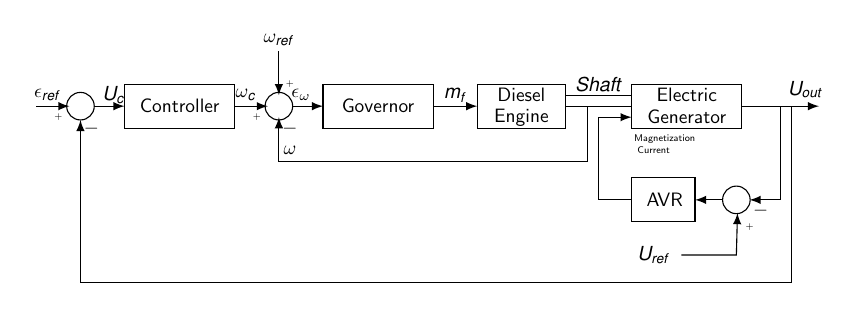
\begin{tikzpicture}[scale=0.7,transform shape]
 \node at (2,0.2) {\normalsize{Governor}};
\draw [-latex] (1,0.6) rectangle (3,-0.2);
 \node at (4.6,0.4) {\normalsize{Diesel}};
  \node at (4.6,0) {\normalsize{Engine}};
\draw [-latex] (3.8,0.6) rectangle (5.4,-0.2);
\draw [-latex](3,0.2) -- (3.8,0.2);
\node at (3.4,0.4) {$m_f$};
 \node at (7.6,0.4) {\normalsize{Electric}};
  \node at (7.6,0) {\normalsize{Generator}};
\draw [-latex] (6.6,0.6) rectangle (8.6,-0.2);

\node at (6,0.6) {$Shaft$};
  \node at (7.2,-1.5) {\normalsize{AVR}};
\draw [-latex] (8.5,-1.5) ellipse (0.25 and 0.25);
\draw [-latex] (6.6,-1.1) rectangle (7.75,-1.9);
\draw [-latex](6.6,-1.5) -- (6,-1.5) -- (6,0) -- (6.6,0);
\node at (8.94,-1.7) {$-$};
\draw [-latex](7.5,-2.5) -- (8.5,-2.5) -- (8.52,-1.74);
\node at (7,-2.5) {$U_{ref}$};
\node at (7.2,-0.4) {\tiny{Magnetization}};
\node at (7,-0.6) {\tiny{Current}};
\node at (9.75,0.5) {$U_{out}$};
\draw [-latex] (0.2,0.2) ellipse (0.25 and 0.25);

\draw [-latex](0.2,1.2) -- (0.2,0.4);
\node at (0.2,1.4) {$\omega_{ref}$};
\draw [-latex](5.8,0.2) -- (5.8,-0.8) -- (0.2,-0.8) -- (0.2,0);
\node at (0.4,-0.6) {$\omega$};
\node at (-1.6,0.2) {\normalsize{Controller}};
\draw [-latex] (-2.6,0.6) rectangle (-0.6,-0.2);
\draw [-latex](-0.6,0.2) -- (0,0.2);
\node at (-0.4,0.4) {$\omega_{c}$};
\draw [-latex] (-3.4,0.2) ellipse (0.25 and 0.25);
\draw [-latex](-3.15,0.2) -- (-2.6,0.2);
\node at (-2.8,0.4) {$U_{c}$};
\draw [-latex](-4.2,0.2) -- (-3.6,0.2);
\node at (-4,0.4) {$\epsilon_{ref}$};
\draw [-latex](9.5,0.2) -- (9.5,-3) -- (-3.4,-3) -- (-3.4,-0.05);
\node at (-3.2,-0.2) {$-$};
\node at (0.6,0.4) {$\epsilon_{\omega}$};
\draw [-latex](9.3,0.2) -- (9.3,-1.5)-- (8.74,-1.5);
\draw [-latex](8.6,0.2) -- (10,0.2);
\draw [-latex](8.244,-1.5) -- (7.75,-1.5);
\draw [thin](5.4,0.2) -- (6.6,0.2);
\draw [thin](5.4,0.4) -- (6.6,0.4);
\draw [thin](0.4,0.2);
\draw [-latex](0.45,0.2) -- (1,0.2);
\node at (-3.8,0) {\tiny{+}};

\node at (8.74,-2) {\tiny{+}};
\node at (0.4,-0.2) {$-$};
\node at (0.4,0.6) {\tiny{+}};
\node at (-0.2,0) {\tiny{+}};
\end{tikzpicture} 
    \vspace{-2mm}
    \captionsetup{font=tiny}
    \captionof{figure}{Block diagram illustrating the genset with an added frequency controller.}
\end{center}

\end{posterbox}

\begin{posterbox}[name=results,span=1,column=2,row=0]{Results}

\end{posterbox}

\begin{posterbox}[name=Control,column=1]{Control}


\begin{center}
    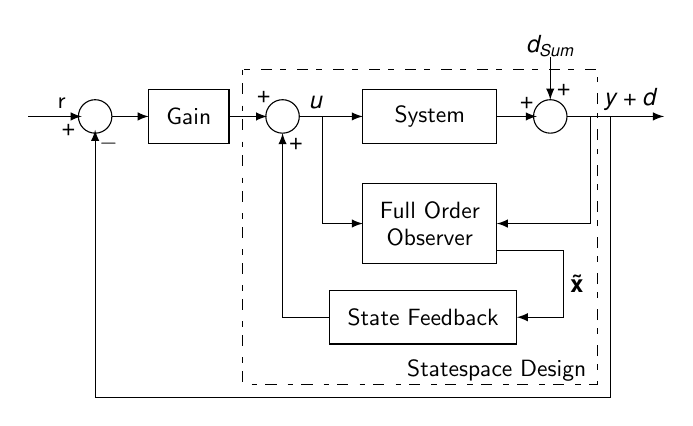
\begin{tikzpicture} [scale=0.85,transform shape]
 \draw [-latex] (-0.2,2) ellipse (0.25 and 0.25);
 \node at (2,2) {\normalsize{System}};
\draw [-latex] (1,2.4) rectangle (3,1.6);
 \node at (2,0.2) {\normalsize{Observer}};
  \node at (2,0.6) {\normalsize{Full Order}};
\draw [-latex] (1,1) rectangle (3,-0.2);
\draw [-latex](0.05,2) -- (1,2);
\draw [-latex](0.4,2) -- (0.4,0.4) -- (1,0.4);
\draw [-latex](4.4,2) -- (4.4,0.4) -- (3,0.4);
 \node at (1.9,-1) {\normalsize{State Feedback}};
\draw [-latex] (0.5,-0.6) rectangle (3.3,-1.4);
  \node at (-1.6,2) {\normalsize{Gain}};
\draw [-latex](-1,2) -- (-0.43,2);
\node at (5,2.25) {\normalsize{$y+d$}};
\node at (0.3,2.2) {\normalsize{$u$}};
\node at (4.2,-0.5) {\normalsize{$\mathbf{\tilde{x}}$}};
\draw [-latex] (-2.2,2.4) rectangle (-1,1.6);
\draw [-latex] (-3,2) ellipse (0.25 and 0.25);
 \draw [-latex] (3.8,2) ellipse (0.25 and 0.25);
\draw [-latex](3,2) -- (3.6,2);
\draw [-latex](4.05,2) -- (5.5,2);
\draw [-latex](-2.75,2) -- (-2.2,2);
\draw [-latex](-4,2) -- (-3.2,2);
\draw [-latex](4.7,2) -- (4.7,-2.2) -- (-3,-2.2) -- (-3,1.8);
 \node at (3.8,3.05) {\normalsize{$d_{Sum}$}};
 \node at (4,2.4) {$+$};
\node at (-2.8,1.6) {$-$};
\node at (-3.4,1.8) {$+$};
\node at (-3.5,2.2) {r };
\draw [dash pattern=on 2pt off 3pt on 4pt off 4pt] (-0.8,2.7) rectangle (4.5,-2);
\node at (3,-1.8) {\normalsize{Statespace Design}};
\node at (-0.48,2.3) {$+$};
\node at (0,1.6) {$+$};
\draw [-latex](0.5,-1) -- (-0.2,-1) -- (-0.2,1.75);
\draw [-latex](3,0) -- (4,0) -- (4,-1) -- (3.3,-1);
\draw [-latex](3.8,2.89) -- (3.8,2.25);
\node at (3.45,2.2) {$+$};
\end{tikzpicture} 
    \vspace{-2mm}
    \captionsetup{font=tiny}
    \captionof{figure}{Block diagram of the control design.}
\end{center}


\end{posterbox}

\begin{posterbox}[name=results_and_simulations,column=1,below=Control]{Results and simulations}

\end{posterbox}

\begin{posterbox}[name=discussion,column=2,below=results]{Discussion}

\end{posterbox}

\begin{posterbox}[name=conclusion,column=2,below=discussion]{Conclusion}

\end{posterbox}

\begin{posterbox}[name=references,column=2,above=bottom]{References}
\bibliography{bibliography}
\end{posterbox}

\end{poster}
\end{document}
